\documentclass[tikz,border=8pt]{standalone}
\usetikzlibrary{shapes.gates.logic.US,positioning}
\begin{document}
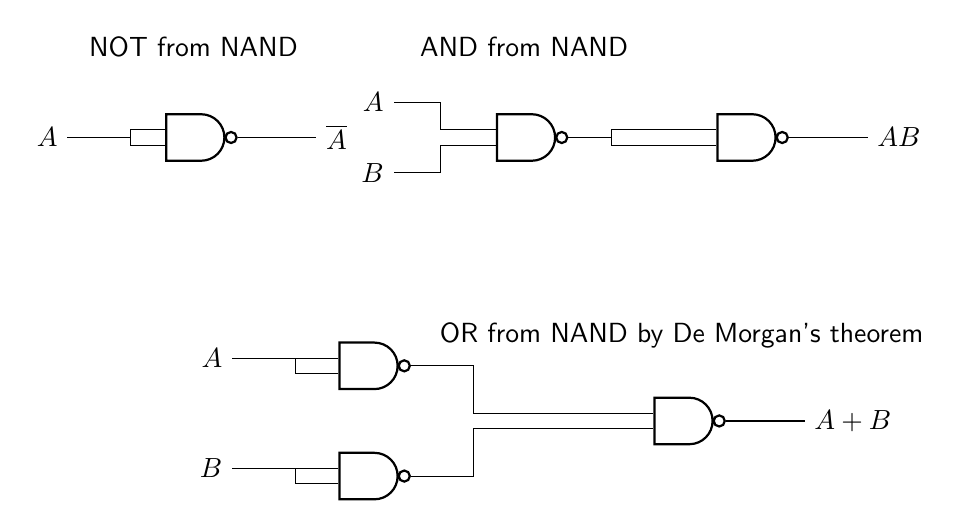
\begin{tikzpicture}[every node/.style={font=\sffamily}, gate/.style={draw,thick,logic gate inputs=nn}]
  \node[nand gate US,gate] (n1) at (0,2.8) {};
  \coordinate (ain) at (-1.6,2.8);
  \draw (ain) node[left]{$A$} -- (-.8,2.8) |- (n1.input 1);
  \draw (-.8,2.8) |- (n1.input 2);
  \draw (n1.output) -- ++(1.0,0) node[right]{$\overline A$};
  \node[above=6mm of n1] {NOT from NAND};

  \node[nand gate US,gate] (n2) at (4.2,2.8) {};
  \node[nand gate US,gate] (n3) at (7.0,2.8) {};
  \draw (n2.input 1) -- ++(-.7,0) -- ++(0,.35) -- ++(-.6,0) node[left]{$A$};
  \draw (n2.input 2) -- ++(-.7,0) -- ++(0,-.35) -- ++(-.6,0) node[left]{$B$};
  \draw (n2.output) -- ++(.55,0) coordinate(xab);
  \draw (xab) |- (n3.input 1);
  \draw (xab) |- (n3.input 2);
  \draw (n3.output) -- ++(1.0,0) node[right]{$AB$};
  \node[above=6mm of n2] {AND from NAND};

  \node[nand gate US,gate] (n4) at (2.2,-.1) {};
  \node[nand gate US,gate] (n5) at (2.2,-1.5) {};
  \node[nand gate US,gate] (n6) at (6.2,-.8) {};
  \draw (n4.input 1) -- ++(-.55,0) coordinate(ia);
  \draw (n4.input 2) -- ++(-.55,0);
  \draw (n4.input 1) ++(-.55,0) |- (n4.input 2);
  \draw (ia) -- ++(-.8,0) node[left]{$A$};
  \draw (n5.input 1) -- ++(-.55,0) coordinate(ib);
  \draw (n5.input 2) -- ++(-.55,0);
  \draw (n5.input 1) ++(-.55,0) |- (n5.input 2);
  \draw (ib) -- ++(-.8,0) node[left]{$B$};
  \draw (n4.output) -- ++(.8,0) |- (n6.input 1);
  \draw (n5.output) -- ++(.8,0) |- (n6.input 2);
  \draw (n6.output) -- ++(1.0,0) node[right]{$A+B$};
  \node[above=5mm of n6] {OR from NAND by De Morgan's theorem};
\end{tikzpicture}
\end{document}
